% VisTacFusion Architecture — v4 (paper-ready, no sub-figures)
% Design: left-to-right, two swim lanes (dense top, pose bottom),
%         arrows encode attention direction, minimal dimensions,
%         frozen = dashed border + snowflake
% Compile: pdflatex -shell-escape architecture_diagram.tex
\documentclass[border=5pt]{standalone}
\usepackage{tikz}
\usepackage{graphicx}
\usepackage{amsmath,amssymb}

\usetikzlibrary{
  arrows.meta, positioning, fit, backgrounds, calc,
  decorations.pathreplacing, shapes.geometric
}

% ── palette (4 hues + gray) ──
\definecolor{cTac}{HTML}{FDEBD0}      % tactile orange
\definecolor{cTacB}{HTML}{E59866}
\definecolor{cVis}{HTML}{D6EAF8}      % visual blue
\definecolor{cVisB}{HTML}{5DADE2}
\definecolor{cTrunk}{HTML}{D5F5E3}    % trunk green
\definecolor{cTrunkB}{HTML}{58D68D}
\definecolor{cDpt}{HTML}{FFF3CD}      % DPT yellow
\definecolor{cDptB}{HTML}{F0C040}
\definecolor{cHead}{HTML}{E8DAEF}     % head purple
\definecolor{cHeadB}{HTML}{AF7AC5}
\definecolor{cOut}{HTML}{F2F3F4}      % output gray
\definecolor{cOutB}{HTML}{808080}
\definecolor{cGate}{HTML}{E57373}     % gated bridge red

\tikzset{
  blk/.style={draw, rounded corners=2pt, align=center,
    font=\footnotesize, inner sep=3pt, line width=0.5pt,
    minimum height=0.75cm},
  frozen/.style={draw, rounded corners=2pt, align=center,
    font=\footnotesize, inner sep=3pt, line width=0.7pt, dashed},
  smallblk/.style={draw, rounded corners=1.5pt, align=center,
    font=\scriptsize, inner sep=2pt, line width=0.4pt,
    minimum height=0.5cm},
  arr/.style={-{Stealth[length=3.5pt,width=2.5pt]}, line width=0.5pt,
    color=black!60},
  garr/.style={-{Stealth[length=3.5pt,width=2.5pt]}, line width=0.6pt,
    dashed, color=cGate},
  lbl/.style={font=\tiny, text=black!50},
  dim/.style={font=\tiny\itshape, text=black!40},
  lane/.style={draw=#1, rounded corners=4pt, line width=0.7pt,
    dashed, inner sep=6pt},
}

\begin{document}
\begin{tikzpicture}[node distance=0.4cm and 0.5cm]

% ====================================================================
% ENCODERS (left)
% ====================================================================

% Tactile encoder
\node[frozen, fill=cTac, draw=cTacB, minimum width=2.0cm,
  minimum height=0.9cm] (enc_t) at (0, 1.0) {
  \textbf{Tactile Enc.}\\[-2pt]
  {\tiny SiTR-B/16}};
\node[font=\tiny, text=cTacB, anchor=south] at (enc_t.north east)
  {\raisebox{0pt}{\fontsize{5}{5}\selectfont\textit{frozen}}};

% Visual encoder
\node[frozen, fill=cVis, draw=cVisB, minimum width=2.0cm,
  minimum height=0.9cm] (enc_v) at (0, -1.4) {
  \textbf{Visual Enc.}\\[-2pt]
  {\tiny MAE-L/16}};
\node[font=\tiny, text=cVisB, anchor=south] at (enc_v.north east)
  {\raisebox{0pt}{\fontsize{5}{5}\selectfont\textit{frozen}}};

% Input thumbnails
\node[inner sep=0, left=0.5cm of enc_t] (img_t)
  {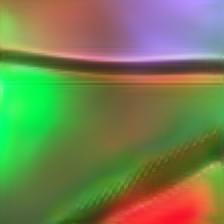
\includegraphics[width=0.9cm]{assets/tactile_sim.png}};
\node[inner sep=0, left=0.5cm of enc_v] (img_v)
  {
\includegraphics[width=0.9cm]{assets/rgb_sim.png}};
\node[below=0.01cm of img_t, font=\tiny\bfseries, text=black!50]
  {Tactile};
\node[below=0.01cm of img_v, font=\tiny\bfseries, text=black!50]
  {RGB};

\draw[arr] (img_t) -- (enc_t);
\draw[arr] (img_v) -- (enc_v);

% ====================================================================
% DENSE PATH (top swim lane)
% ====================================================================

% Multiscale taps — 4 stacked rectangles suggesting different scales
\node[blk, fill=cDpt!60, draw=cDptB, minimum width=1.6cm,
  minimum height=0.95cm] (taps) at (3.0, 2.7) {
  \textbf{Multiscale}\\[-2pt]\textbf{Taps}\\[-2pt]
  {\tiny 4 layers}};

% Gated injection
\node[blk, fill=cDpt!40, draw=cDptB, minimum width=1.8cm,
  minimum height=0.75cm] (inject) at (5.6, 2.7) {
  \textbf{Gated Inject.}\\[-2pt]
  {\tiny $\alpha_{\mathrm{init}}{=}0$}};

% DPT decoder — show as cascade
\node[blk, fill=cDpt, draw=cDptB, minimum width=1.8cm,
  minimum height=0.75cm] (dpt) at (8.4, 2.7) {
  \textbf{DPT Decoder}\\[-2pt]
  {\tiny reassemble $\to$ fuse}};

% Outputs
\node[blk, fill=cOut, draw=cOutB, minimum width=1.0cm,
  font=\scriptsize] (depth) at (10.5, 3.1) {Depth};
\node[blk, fill=cOut, draw=cOutB, minimum width=1.0cm,
  font=\scriptsize] (normal) at (10.5, 2.3) {Normal};

% Output thumbnails
\node[inner sep=0, right=0.1cm of depth] (depth_img)
  {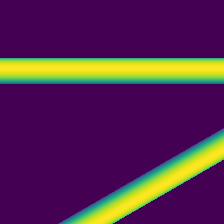
\includegraphics[width=0.6cm]{assets/depth_gt.png}};
\node[inner sep=0, right=0.1cm of normal] (normal_img)
  {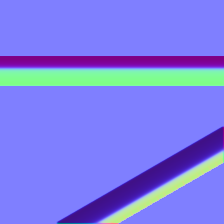
\includegraphics[width=0.6cm]{assets/normal_gt.png}};

% Dense path arrows
\draw[arr] (taps) -- (inject);
\draw[arr] (inject) -- (dpt);
\draw[arr] (dpt.east) -- ++(0.12,0) |- (depth.west);
\draw[arr] (dpt.east) -- ++(0.12,0) |- (normal.west);

% Encoder → taps
\draw[arr, color=cTacB] (enc_t.north) -- ++(0, 0.7)
  -| (taps.south)
  node[pos=0.25, right=1pt, lbl] {intermediate features};

% ====================================================================
% POSE PATH (bottom swim lane)
% ====================================================================

% Projections (small)
\node[smallblk, fill=cTac!30, draw=cTacB!50,
  minimum width=1.1cm] (proj_t) at (2.6, 0.15) {
  \textbf{Proj}\\[-2pt]{\tiny 768→768}};
\node[smallblk, fill=cVis!30, draw=cVisB!50,
  minimum width=1.1cm] (proj_v) at (2.6, -1.4) {
  \textbf{Proj}\\[-2pt]{\tiny 1024→768}};

\draw[arr, color=cTacB!70] (enc_t.east) -- ++(0.15,0)
  |- (proj_t.west);
\draw[arr, color=cVisB!70] (enc_v.east) -- (proj_v.west);

% Queries & Memory
\node[smallblk, fill=cTac!20, draw=cTacB!40,
  minimum width=1.4cm] (queries) at (4.4, 0.15) {
  \textbf{Tactile Queries}\\[-2pt]{\tiny 197 tokens}};
\node[smallblk, fill=cVis!20, draw=cVisB!40,
  minimum width=1.4cm] (memory) at (4.4, -1.4) {
  \textbf{Visual Memory}\\[-2pt]{\tiny 197 tokens}};

\draw[arr] (proj_t) -- (queries);
\draw[arr] (proj_v) -- (memory);

% ====================================================================
% FUSION TRUNK — visual bottleneck metaphor
% ====================================================================

% Trunk outer box
\node[blk, fill=cTrunk!40, draw=cTrunkB,
  minimum width=3.0cm, minimum height=2.6cm] (trunk) at (7.4, -0.6) {};

% Title
\node[font=\footnotesize\bfseries, text=cTrunkB!70!black,
  anchor=north] at (trunk.north) {Fusion Trunk};
\node[dim, anchor=north] at ($(trunk.north)+(0,-0.30)$) {$\times\,4$ layers};

% Bottleneck strip (narrow = visual metaphor for compression)
\node[blk, fill=cTrunk!80, draw=cTrunkB, minimum width=0.7cm,
  minimum height=0.55cm, font=\tiny, inner sep=1.5pt]
  (bn) at ($(trunk.center)+(0, 0.25)$) {
  \textbf{BN}\\[-1pt]{\fontsize{4.5}{5}\selectfont $m{=}16$}};

% Attention steps as compact labels
\node[font=\tiny, text=black!65, align=left, anchor=north west]
  at ($(trunk.south west)+(0.15, 0.72)$) {
  \textcircled{\fontsize{4}{4}\selectfont 1}\;Mem $\to$ BN\\[2pt]
  \textcircled{\fontsize{4}{4}\selectfont 2}\;BN\phantom{e} $\to$ Q\\[2pt]
  \textcircled{\fontsize{4}{4}\selectfont 3}\;Q self-attn};

% Queries → trunk (left side, upper)
\draw[arr, color=cTacB!60] (queries.east) -- ++(0.15,0)
  |- ($(trunk.west)+(0, 0.0)$)
  node[pos=0.75, above=1pt, lbl] {Q};

% Memory → trunk (left side, lower)
\draw[arr, color=cVisB!60] (memory.east) -- ++(0.15,0)
  |- ($(trunk.west)+(0, -0.8)$)
  node[pos=0.75, above=1pt, lbl] {KV};

% ====================================================================
% POSE HEAD
% ====================================================================

\node[blk, fill=cHead!70, draw=cHeadB, minimum width=1.1cm,
  minimum height=0.6cm, font=\scriptsize] (pose_mlp)
  at (10.0, -1.4) {\textbf{Pose MLP}};

\node[blk, fill=cOut, draw=cOutB, minimum width=1.0cm,
  font=\scriptsize] (se2) at (11.5, -1.4) {
  \textbf{SE(2)}\\[-2pt]{\tiny $\theta, t_x, t_y$}};

\draw[arr] ($(trunk.east)+(0, -0.8)$) -- (pose_mlp.west)
  node[midway, below=1pt, lbl] {pose token + pool};
\draw[arr] (pose_mlp) -- (se2);

% ====================================================================
% BRIDGE: Bottleneck → Gated Injection (the cross-path link)
% ====================================================================

\draw[garr, line width=0.6pt]
  ($(trunk.north)+(-0.3, 0)$) -- ++(0, 1.05)
  -| (inject.south)
  node[pos=0.5, above=1pt, font=\tiny, text=cGate!80!black]
    {visual context $B_4$};

% ====================================================================
% LANE LABELS (background, no boxes — just text)
% ====================================================================

\begin{scope}[on background layer]
  % Dense lane highlight
  \node[lane=cDptB!50, fill=cDpt!8,
    fit=(taps)(inject)(dpt)(depth)(normal)(depth_img)(normal_img),
    label={[font=\scriptsize\bfseries, text=cDptB!60!black,
      anchor=north west, xshift=3pt, yshift=-1pt]
      north west:Dense path}] {};
  % Pose lane highlight
  \node[lane=cTrunkB!50, fill=cTrunk!6,
    fit=(proj_t)(proj_v)(queries)(memory)(trunk)(pose_mlp)(se2),
    label={[font=\scriptsize\bfseries, text=cTrunkB!60!black,
      anchor=south west, xshift=3pt, yshift=1pt]
      south west:Pose path}] {};
\end{scope}

% ====================================================================
% MINIMAL ANNOTATIONS
% ====================================================================

% Modality dropout
\node[font=\tiny, text=black!35, anchor=north east]
  at ($(se2.south east)+(0.1, -0.05)$)
  {modality dropout (pose path)};

\end{tikzpicture}
\end{document}
